\documentclass[11pt, letterpaper]{article}

\usepackage[english]{babel}
\usepackage[utf8x]{inputenc}
\usepackage[gen]{eurosym}
\usepackage{amsmath}
\usepackage{amssymb}
\usepackage[dvipsnames]{xcolor}
\usepackage{graphicx}
\usepackage[stable]{footmisc}
\usepackage{caption}
\usepackage{subcaption} 
\usepackage[title]{appendix}
\usepackage{multirow}
\usepackage{xcolor}
\usepackage[margin=1.0in]{geometry}
\usepackage{array}
%\usepackage{hyperref}

\usepackage{tablefootnote}
\usepackage{lineno}
\usepackage{pifont}% http://ctan.org/pkg/pifont
\newcommand{\cmark}{\ding{51}}%
\newcommand{\xmark}{\ding{55}}%

\captionsetup{font=footnotesize}

\newcommand\boldred[1]{\textcolor{red}{\textbf{#1}}}
\newcommand{\seba}{\textcolor[rgb]{0,1,1}}
\newcommand{\fel}[1]{{\color{red}({\bf FF:}#1)}}
\newcommand{\pia}{\textcolor[rgb]{0,0,1}}


 
\title{Cap-and-trade Model for the Chilean Energy Market}
\author{P\'ia Amigo, Sebasti\'an Cea, Felipe Feijoo}
\date{\today}

\begin{document}
\linenumbers
\maketitle

\section{Motivation}

Considerar un mercado de cap-and-trade como opción a incrementar el tax en chile\footnote{pag 64. https://mma.gob.cl/wp-content/uploads/2015/09/hojaderuta.pdf}



\section{Model}\label{model}

Let us consider a market of $N$ producers indexed by $i\in\{1,...,N\}$, each of them minimizing the cost of operation and investment. We will assume perfect competition among the producers. Our model will assume two basic stages: operation today and investment for the future in period $t=0$ and the uncertain future where there is a spot market and trade of emission allowances in periods $t\in T:=\{1,...\bar{t}\}$. Uncertainty is revealed in period $t=1$ and is represented by a state of nature $\omega\in\Omega:=\{1,..,K\}$. Thus, for a given state of nature $\omega\in\Omega$, the pair $(t,\omega)$ represents the future in period $t$ when the state $\omega$ is achieved.

\smallskip

At first stage, we consider the present operating plant of the producer $i$, the cost of the operation $C_i$, and the quantity produced $Q_i(t)$ with $t=0$. The selling price (that satisfies the demand) at this stage is $\pi^d(t)$ with $t=0$. The maximum quantity of production at current stage ($t=0$) per producer is $\bar{Q}_i$. Each producer buys a certain amount of carbon allowances $A_i\in\mathbb{R}_+$ at a price $\pi^{a}$ from an auctioneer or regulatory agent.  The auctioneer will try to maximize the revenue obtained from the sold allowances. At this stage when $t=0$, the producer $i$ decides the amount $x_i(t)$ of capacity expansion at a cost $I_i$ for the uncertain future.

\smallskip

At the second stage for each $t\in T$ and given $\omega\in \Omega$, the producer wants to operate in the most efficient way at the spot market choosing production level $Q_i(t,\omega)\in\mathbb{R}_+$ with a cost  $TC_i(t,\omega)\cdot C_i$ where $TC_i(t,\omega)\in\mathbb{R}_+$ is the change of the cost. Also, the producer can invest in a capacity expansion $x_i(t,\omega)\in\mathbb{R}_+$ with an investment cost of $TCR_i(t,\omega)I_i$  where $TCR_i(t,\omega)\cdot C_i$ the change in the investment cost. In addition,  we will consider the existence of a permit trading system, where producers can purchase $P_i(t,\omega)\in\mathbb{R}_+$ permits from other producers if they need to surpass the emission allowances $A_i$, or sell $V_i(t,\omega)\in\mathbb{R}_+$ unused permits if their emissions are below allowances $A_i$. The price of transaction in this system is $\pi^v(t,\omega)$. The producer will evaluate the cost of the uncertain future as a risk neutral agent, i.e., expectated value with a probability obtained from real world data.
\smallskip


The maximum budget for emissions is denoted by  $CAP\in\mathbb{R}_+$ and is drawn from a normal distribution, i.e., $CAP \thicksim N(\mu, \sigma^2)$. This $CAP$ is determined by the auctioneer and  accounts for the total emissions throughout the whole period considered, that is, does not depend on $t$. 


\smallskip
The amount of total allowances provided by the auctioneer, $\theta\in\mathbb{R}_+$, is an endogenous variable in our model, and it must satisfy the condition $\sum_i A_i \leq \theta$. 
Since $\theta$ must not surpass the budget for emissions, we consider a small margin of risk given by a probability bound $M\in(0,1)$ for this to happen, i.e.,
\begin{equation}
    Pr(\theta \geq CAP) \leq M,
\end{equation}

and since the variable $CAP$ is chosen from a normal distribution with mean $\mu$ and variance $\sigma^2$, we can write the equation above as
\begin{equation}
    \theta \leq \phi^{-1}(M) \sigma^2 + \mu
\end{equation}

where $\phi^{-1}$ is the inverse of the cumulative function of the normal distribution. 


\hspace{0.5cm}




\subsection{Producer's problem}

Each producer $i$ represents one and only one technology in the economy. The choice set of the producer $i$ over a time horizon of $\bar{t}$ years is given by: i) an amount of capacity expansion $x_i:=\left(x_i(0),x_i(t,\omega)_{(t,\omega)\in T\times\Omega}\right)\in\mathbb{R}_+\times\mathbb{R}_+^{T\times\Omega}$, ii) a production plan $Q_i:=\left(Q_{i}(0),(Q_{i}(t,\omega)_{(t,\omega)\in T\times\Omega}\right)\in\mathbb{R}_+\times\mathbb{R}_+^{T\times\Omega}$, iii) allowances bought in the first period $A_i\in\mathbb{R}_+$, iv) allowances bought in the second period $P_i(t,\omega)\in\mathbb{R}_+^{T\times\Omega}$ and v) allowances sold in the second period $V_i(t,\omega)\in\mathbb{R}_+^{T\times\Omega}$.

We define the cost function for $t\in T_0:=\{0\}\cup T$ by

$$C_i(t,\pi^{d}(t),Q_i(t))={\color{red}\Big(a_iQ_i(t)+\frac{b}{2}Q_i(t)^{2}\Big)-\pi^{d}(t) Q_i(t)}.$$


%_{\seba{\left(C_t^{comb}\cdot C^{esp}+CVnC\right)Q_{i,t}+\underbrace{FixedCost_{i,t}}_{\frac{\alpha\cdot I\cdot x}{algo}}}}

%and for the rest of the periods

%$$C_i(t,\pi^{d}(t),Q_i(t,\omega))={\color{red}\Big(a_iQ_i(t)+\frac{b}{2}Q_i(t)^{2}\Big)-\pi_{d}(t) Q_i(t,\omega)}$$

Therefore the objective function of producer $i$ is given by

\begin{align}
\min_{(x_i,Q_i,A_i,P_i,V_i)\in (\mathbb{R}_+^{T_0\times\Omega} \times\mathbb{R}_+^{T_0\times\Omega} \times \mathbb{R}\times\mathbb{R}_+^{T\times\Omega}\times\mathbb{R}_+^{T\times\Omega})} &  C_i(0, \pi^d(0),Q_i(0))+ A_i \pi^{a} + I_i x_i(0) \nonumber \\ &+\sum_{\omega} Pr(\omega)   \Bigg( \sum_{t>0} \frac{1}{(1+R)^t} \Big[ (TC_i(t,\omega)\cdot C_i(t,\pi^d(t),Q_i(t,\omega) )  \nonumber \\
 & + \sum_{t > 0} TCR_i(t,\omega) \cdot I_i\cdot x_i(t,\omega) \Big] + \pi^v(t,\omega)\cdot \left(P_i(t,\omega)-V_i(t,\omega)\right) \Bigg)  \label{prodFO} \\
     \textrm{s.t \ } \nonumber
\end{align}
\begin{align}
    \Big(CF_i \cdot\tau\Big)  \Bigg[\bar{Q_i} + \sum_{t^{\prime}<\bar{t}} x_i(t^\prime,\omega) + x_i(0)+ \bar{Q}_i(t) \Bigg] - Q_i(t,\omega) & \geq 0  & \forall  \quad \omega, t  > 0 & \quad (\alpha_{i,\omega,t}) \\
    \Big(CF_i\cdot\tau \Big)\bar{Q_i}-Q_{i}(0) & \geq 0  &  \quad & \quad (\kappa_i) \\
 A_{i} -V_i(t,\omega) & \geq  0  & \forall  \quad t,\omega & \quad (\beta_{i,\omega})\\
 A_{i} + \sum_{i}P_i(t,\omega) - V_i(t,\omega)-\sum_{t>0}Q_i(t, \omega)\cdot \varepsilon_{i}-Q_i(0)\varepsilon_{i} & \geq  0  &\forall \quad t,\omega & \quad (\gamma_{i,\omega})\\
 Q_i(0) & \geq  0 & \quad & \quad (\lambda_i)\\
 Q_i(t, \omega & \geq  0   & \forall  \quad \omega, t >0 & \quad (\delta_{i,\omega})\\
  x_i(0) & \geq  0 & \quad & \quad (\xi_i)\\
  x_i(t, \omega) & \geq  0   & \forall  \quad \omega, t >0 & \quad (\varphi_{i,\omega,t})\\
{\color{blue} RP_i - \bar{Q}_i - \bar{Q}_i(t) - x_i(0) - \sum_{t > 0} x_i(t,\omega) } & {\color{blue} \geq 0} & {\color{blue} \forall \quad i,\omega }&  {\color{blue} \quad (\psi_{i,\omega}) }
  \end{align}\\

\subsection{Equilibrium}


\subsection{Computation}

\begin{center}
\begin{tabular}{ l l  } 
 \hline
 \textbf{Set} &  \textbf{Explanation} \\ 
 \hline
 \hline
 $i$ & Producers (Technologies) \\  
 $\omega$ & Possible scenarios \\ 
 $t$ & Periods \\
 \hline
\end{tabular}
\end{center}

For this model, each producer corresponds to a different technology present in the chilean electricity generation system, i.e., Biomasa, Carbon, Eolica, Gas, Geotermica, HidroEmbalse, HidroPasada, HidroMiniPasada, PetroleoDiesel, Solar.

\begin{center}
\begin{tabular}{  l l l l  } 
 \hline
 \textbf{Parameter} & \boldred{Suggested} & \textbf{Units} & \textbf{Explanation} \\ 
 \hline
 \hline
 $I_i$ & & USD/MW & Expansion cost per technology $i$ \\  
 $\bar{Q}_i$ & \boldred{$\bar{X}_i$} & MW & Maximum operation capacity per technology $i$  \\ 
 $C_i$ &  & USD/MWh & Operation cost per technology $i$ \\
 $D^{1}$ & & MWh & Total demand in first stage \\
 $D^{t}_{\omega}$ & & MWh & Total demand in period $t > 1$ \\
 $\varepsilon_i$ & & tCO$_{2}$/MWh  & Emission factor of technology $i$\\
 Prob$_\omega$ & \boldred{$\Pi_\omega$} & & Physical probability of scenario $\omega$ \\
 $\mu$ & & tCO$_{2}$ & Mean of the normal distribution of the CAP \\
  $\sigma$ & & tCO$_{2}$ & Standard deviation of the normal distribution of the CAP \\
  $\epsilon$ & &  & Margin for total emission allowances \\
  $R$ & \boldred{df} & & Discount rate \\
  $TC_i$ & & & Change in the cost of operation per technology \\
  $TCR_i$ & & & Change in the investment cost per technology \\
  $CF_i$ & & & Capacity factor per technology\\
  $\tau$ & & hours&  Number of hours in a year, $\tau=8760$ hours\\
  {\color{blue} $RP_i$ } & & {\color{blue} MW} & {\color{blue} Resource potential per technology }\\
\hline
\end{tabular}
\end{center}

\begin{center}
\begin{tabular}{  l l l l  } 
 \hline
 \textbf{Variable} & \boldred{Suggested} & \textbf{Units} & \textbf{Explanation} \\ 
 \hline
 \hline
 $Q^{1}_i$ & \boldred{$Y^{1}_{i}$} & MWh & produced quantity in period $t =1  $ for producer $i$\\
 $Q^{t}_{i,\omega}$ & \boldred{$Y^{t}_{i,\omega}$} & MWh & produced quantity in period $t > 1 $ for producer $i$ in scenario $\omega$ \\  
 $A_i$ & \boldred{$\theta_i$} & tCO$_2$ & Emission allowances purchased by producer $i$ \\ 
 $P_{i,j,\omega}$ & \boldred{$B_i$}& tCO$_2$ & Purchased permits in trading market by producer i  \\
 $V_{i,\omega}$ & & tCO$_2$ & Sold permits in trading markets \\
 $\pi^{a}$ & \boldred{$P^{a}$} & USD/tCO$_2$  & Price of the allowances offered by the auctioneer (dual to CAP constraints)\\
 $\pi^{v}_{i,\omega}$ & \boldred{$P^{v}_{i,\omega}$} & USD/tCO$_2$  & Price of the permits in trading market (dual to trading equilibrium)\\
  $\pi^{d,1}$ & \boldred{$P^{d,1}$} & USD/MWh  & Price of electricity (dual to fulfilment of the demand --first stage)\\
 $\pi^{d,t}_{\omega}$ & \boldred{$P^{d,t}$} & USD/MWh  & Price of electricity (dual to fulfilment of the demand)\\
 $x^{1}_i$ & & MW  & Capacity expansion decision for period $t=1$ of producer $i$\\
 $x^{t}_{i,\omega}$ & & MW  & Capacity expansion decision for period $t$ of producer $i$ in scenario $\omega$\\
  $\theta$ & \boldred{$\Theta$} & tCO$_2$ & Emission allowances available in the market by the auctioneer\\
\hline
\end{tabular}
\end{center}

\vspace{0.5cm}


\underline{Producer's problem} (each producer is a different technology):

\small
\begin{align}
\min_{x,Q,A,P,V} & \underbrace{{\color{red}\Big(a_iQ_{1,i}+\frac{b}{2}Q_{1,i}^{2}\Big)-\pi^{d,1} Q_{1,i}}}_{\seba{\left(C_t^{comb}\cdot C^{esp}+CVnC\right)Q_{i,t}+\underbrace{FixedCost_{i,t}}_{\frac{\alpha\cdot I\cdot x}{algo}}}} + A_i \pi^{a} + I_i x_i^{1} + \sum_{\Omega} prob_\omega   \Bigg( \sum_{t>1} \frac{1}{(1+R)^t} \Big[ (TC_{i,\tau}\cdot {\color{red}(a_i Q_{i,t,\omega}+\frac{b}{2}Q_{i,t,\omega}^{2})}\nonumber \\
    & {\color{red}-\pi^{d,2}_{\omega} Q_{i,t,\omega}} + \sum_{t > 1} TCR_i \cdot I_ix^{t}_{i,w} \Big] - V_{i,\omega}\pi_{i,w}^v+\sum_{j\neq i}  P_{i,j,\omega}\pi_{j,w}^v\Bigg)  \\
     \textrm{s.t \ } \nonumber
\end{align}
\begin{align}
    \Big(CF_i \cdot\tau\Big)  \Bigg[\bar{Q_i} + \sum_{t^{\prime}<t_{y_i}} x^{t^{\prime}}_{i,w} + x_i^{1}+ \bar{Q}_{i,t} \Bigg] - Q_{i,\omega}^{t} & \geq 0  & \forall  \quad \omega, t  > 1 & \quad (\alpha_{i,\omega,t}) \label{const.1}\\
    \Big(CF_i\cdot\tau \Big)\bar{Q_i}-Q_{i}^{t} & \geq 0  &  \quad t  =1 & \quad (\kappa_i) \label{const.2} \\
 A_{i} -V_{i,\omega} & \geq  0  & \forall  \quad \omega & \quad (\beta_{i,\omega})\\
 A_{i} + \sum_{j \neq i}P_{i,j,\omega} - V_{i,\omega}-\sum_{t>1}Q_{i, \omega}^{t}\varepsilon_{i}-Q_i^{1}\varepsilon_{i} & \geq  0  &\forall \quad \omega & \quad (\gamma_{i,\omega})\\
 Q_i^{1} & \geq  0 & \quad & \quad (\lambda_i)\\
 Q_{i, \omega}^{t} & \geq  0   & \forall  \quad \omega, t >1 & \quad (\delta_{i,\omega})\\
  x_i^{1} & \geq  0 & \quad & \quad (\xi_i)\\
  x_{i, \omega}^{t} & \geq  0   & \forall  \quad \omega, t >1 & \quad (\varphi_{i,\omega,t})\\
{\color{blue} RP_i - \bar{Q}_i - \bar{Q}_{i,t} - x^{1}_i - \sum_{t > 1} x^{t}_{i,w} } & {\color{blue} \geq 0} & {\color{blue} \forall \quad i,\omega }&  {\color{blue} \quad (\psi_{i,\omega}) }
  \end{align}\\
\normalsize  
  
 
 (\textbf{FELIPE}: Note that $C_i\seba{(Q_i)}$ represents the \seba{marginal} cost function of producer $i$. We consider quadratic \seba{marginal} cost functions of the form $C_i\seba{(Q_i)}=a+\frac{b}{2}Q\seba{_i}$. Hence, I have rewritten the model formulation to account for this change)

The units of each parameter and variable in Equation (\ref{prodFO}) must be suitable such that the objective function has units of cost (us\$). In Equations (\ref{const.1}) and (\ref{const.2}) the factor $CF_i \cdot \tau$ is added to take into account the real production of electricity.\\

\underline{Auctioneer's problem:}

\begin{align}
    \min_{\theta} & -\theta \pi^{a} \\
    \textrm{s.t \ } &  \phi^{-1}(\epsilon) \sigma^2 + \mu - \theta  \geq 0\\
    &  \theta  \geq 0
\end{align}
\vspace{0.5cm}

\underline{Market clearing constraints:}

\begin{align}
\textrm{(available allowances)}: &  \ \   \sum_{i} A_{i} = \theta   &  & \ \  (\pi^{a})\\
\textrm{(equilibrium in trading market)}: &   \ \  \sum_{i, j\neq i} P_{j,i,\omega} = \sum_{i} V_{i,\omega} & \forall \ \omega & \ \ (\pi^{v}) \\
\textrm{(fulfillment of the demand --first stage)}:  &   \ \  \sum_{i} Q^{1}_i = D^{1}, &  & \ \ (\pi^{d,1})\\
\textrm{(fulfillment of the demand --second stage)}:  &   \ \  \sum_{i} Q^{t}_{i,\omega} = D^{t}_{\omega}, & \forall \ \omega, \tau & \ \ (\pi^{d,t}_\omega)
\end{align}

\vspace{0.5cm}

The Lagrangian function for the producer's problem of each $i \in \{ 1,...,n\}$ is:

\begin{align}
    \mathcal{L}_i(x,Q,A,P,V) = &  {\color{red}(a_iQ_{1,i}+\frac{b}{2}Q_{1,i}^{2})-\pi^{d,1} Q_{1,i}}  + A_i \pi^{a} + I_i x_i^{1}  + \sum_{\Omega} prob_\omega  \Bigg( \sum_{t>1} \frac{1}{(1+R)^t} \Big[ (TC_{i}\cdot {\color{red}(a_iQ_{i,t,\omega}+\frac{b}{2}Q_{i,t,\omega}^{2})}\nonumber \\
    & {\color{red}-\pi^{d,2}_{\omega}) Q_{i,t,\omega}} \nonumber \\
    & + \sum_{t > 1} TCR_i \cdot I_ix^{t}_{i,\omega} \Big]  - V_{i,\omega}\pi_{i,\omega}^v+\sum_{j\neq i}  P_{i,j,\omega}\pi_{j,\omega}^v\Bigg) + \kappa_{i}\Big[Q_{i}^{1} -  \Big(CF_i\cdot\tau \Big)\bar{Q_i}\Big] \nonumber \\ 
   &  +\sum_{\omega,t>1} \alpha_{i,\omega,t}\Bigg[Q_{i,\omega}^{t} - \Big(CF_i \cdot\tau\Big) \Big(\bar{Q_i} +\bar{Q}_{i,t}+ \sum_{t^{\prime}<= t } x^{t}_{i,w} + x_i^{1} \Big)\Bigg]  + \sum_{\omega}\beta_{i,\omega}\Big[V_{i,\omega}-A_i\Big]  \nonumber \\
   & + \sum_{\omega}\gamma_{i,\omega} \Big[-A_{i} - \sum_{j \neq i}P_{i,j,\omega} + V_{i,\omega}+\sum_{t>1}Q_{i, \omega}^{t}\varepsilon_{i}+Q_i^{1}\varepsilon_{i}\Big] \nonumber\\
     & - \sum_{\omega, t>1}\delta_{i,\omega,t} Q_{i,\omega}^{t} - \lambda_{i}\Big[Q^{1}_{i}\Big] - \sum_{\omega, t>1}\varphi_{i,\omega,t} x_{i,\omega}^{t} - \xi_i x^{1}_i {\color{blue} + \sum_{\omega}\psi_{i,\omega} \Big[  \bar{Q}_i+\bar{Q}_{i,t} + x^{1}_i + \sum_{t > 1} x^{t}_{i,w} - RP_i \Big]}
\end{align}



where $\alpha_{i,\omega,\tau}$, $\kappa_i$, $\beta_{i,\omega}$, $\gamma_{i,\omega}$ and $\delta_{i,\omega}$  $\lambda_i$, $\varphi_{i,\omega,t}$ ad $\xi_i$ are the lagrange multipliers of the constraints. \newline

The KKT conditions of the producer's problem are then

\begin{align}
    I_i {\color{blue} + \sum_{\omega}\psi_{i,\omega}} -\sum_{\omega,\tau>1} \alpha_{i,\omega,\tau} -\xi_i & = 0 & \forall i {\color{blue}}&  \qquad (x^{1}_{i})\\
    prob_\omega \Bigg[\frac{1}{(1+R)^t}TCR_i \cdot I_i -  \varphi_{i,\omega,t}\Bigg] - \sum_{t> t\prime}\alpha_{i,\omega,t} ( CF_i \cdot \tau) {\color{blue} + \psi_{i,\omega}}& = 0 & \forall i, \omega, t> 1  &  \qquad (x^{t}_{i,\omega})\\
    {\color{red}(a_{i}+b_iQ^{1}_{i})}-(\pi^{d,1}) + \kappa_i - \lambda_{i} + \sum_{\omega} \gamma_{i,\omega}\varepsilon_i & = 0 & \forall i  &  \qquad (Q^{1}_{i})\\
    prob_\omega \Bigg( \frac{1}{(1+R)^t}\Bigg) ( {\color{red}(TC_i \cdot a_{i}+b_iQ_{i,\omega}^{\tau})}-\pi^{d,t}_{\omega}) + \alpha_{i,\omega,\tau} + \gamma_{i,\omega} \varepsilon_{i}-\delta_{i,\omega,\tau} & =0 & \forall i, \omega, \tau>1 &  \qquad (Q_{i,\omega}^{\tau})\\
    \pi^{a} - \sum_{\omega}\beta_{i,\omega} - \sum_{\omega}\gamma_{i,\omega} & =0 & \forall i & \qquad (A_{i}) \\
    -prob_\omega \pi^v_{i,\omega} + \beta_{i,\omega}  + \gamma_{i,\omega} & =0 & \forall i, \omega & \qquad (V_{i,\omega}) \\
    prob_\omega \pi^v_{j,\omega} -\gamma_{i,\omega} & = 0 & \forall i, j \neq i ,\omega & \qquad (P_{i,j,\omega})
\end{align}

\smallskip


\begin{flushleft}
Primal feasibility
\end{flushleft}

\begin{align}
\big(CF_i \cdot \tau \big) \Bigg[\bar{Q_i} + \sum_{t\leq t^{\prime}} x^{t}_{i,w} + x_i^{1} \Bigg] - Q_{i,\omega}^{t} & \geq 0  & \forall  \quad \omega, t  > 1 & \quad (\alpha_{i,\omega,t}) \\
    \Big(CF_i\cdot\tau \Big)\bar{Q_i}-Q_{i}^{t} & \geq 0  &  \quad t  =1 & \quad (\kappa_i) \\
 A_{i} -V_{i,\omega} & \geq  0  & \forall  \quad \omega & \quad (\beta_{i,\omega})\\
 A_{i} + \sum_{j \neq i}P_{i,j,\omega} - V_{i,\omega}-\sum_{t>1}Q_{i,\omega}^{t}\varepsilon_{i}-Q_i^{1}\varepsilon_{i} & \geq  0  &\forall \quad \omega & \quad (\gamma_{i,\omega})\\
 Q_i^{1} & \geq  0 & \quad & \quad (\lambda_i)\\
 Q_{i, \omega}^{t} & \geq  0   & \forall  \quad \omega, t >1 & \quad (\delta_{i,\omega})\\
  x_i^{1} & \geq  0 & \quad & \quad (\xi_i)\\
  x_{i, \omega}^{t} & \geq  0   & \forall  \quad \omega, t >1 & \quad (\varphi_{i,\omega,t})\\
  {\color{blue} RP_i - \bar{Q}_i - x^{1}_i - \sum_{t>1} x^{t}_{i,w} } & {\color{blue} \geq 0} & {\color{blue} \forall \quad i,\omega }&  {\color{blue} \quad (\psi_{i,\omega}) }
\end{align}

\smallskip

\begin{flushleft}
Complementary slackness
\end{flushleft}

\begin{align}
    \Bigg( \big(CF_i \cdot \tau \big) \Bigg[\bar{Q_i} + \sum_{t\leq t^{\prime}} x^{t}_{i,w} + x_i^{1} \Bigg] - Q_{i,\omega}^{t} \Bigg) \cdot \alpha_{i,\omega,\tau} & = 0 & \forall  \quad \omega, t  > 1\\
    \Bigg( \Big(CF_i\cdot\tau \Big)\bar{Q_i}-Q_{i}^{t} \Bigg)\cdot \kappa_i & = 0  & \quad t  =1 \\
    \Bigg(  A_{i} -V_{i,\omega} \Bigg) \cdot \beta_{i,\omega} & = 0 & \forall  \quad \omega\\
    \Bigg( A_{i} + \sum_{j \neq i}P_{i,j,\omega} - V_{i,\omega}-\sum_{t>1}Q_{i,\omega}^{t}\varepsilon_{i}-Q_i^{1}\varepsilon_{i}\Bigg)\cdot \gamma_{i,\omega} & = 0 & \forall \quad \omega \\
    \Bigg( Q_i^{1} \Bigg) \cdot \lambda_i & = 0 & \\
    \Bigg(Q_{i,\omega}^{\tau}\Bigg ) \cdot \delta_{i,\omega} & = 0 & \forall  \quad \omega, t >1\\
    \Bigg( x_i^{1} \Bigg) \cdot \xi_i & = 0 & \\
    \Bigg( x_{i, \omega}^{t} \Bigg) \cdot \varphi_{i,\omega,t} & = 0 & \forall  \quad \omega, t >1 \\
    {\color{blue} \Bigg(RP_i - \bar{Q}_i - x^{1}_i - \sum_{t>1} x^{t}_{i,w}  \Bigg) \cdot \psi_{i,\omega}}&  {\color{blue} = 0 }&  {\color{blue} \forall \quad i,\omega }
\end{align}

\smallskip

\begin{flushleft}
Dual Feasibility
\end{flushleft}

\begin{align}
    \alpha_{i,\omega,\tau} & \geq 0 \\
    \kappa_i & \geq 0 \\
    \beta_{i,\omega} & \geq 0 \\
    \gamma_{i,\omega} & \geq 0 \\
    \lambda_i & \geq 0 \\
    \delta_{i,\omega,t} & \geq 0 \\
    \xi_i & \geq 0 \\
    \varphi_{i,\omega,t} & \geq 0 \\
    {\color{blue}\psi_{i,\omega}} & {\color{blue} \geq 0}
\end{align}

For the Auctioneer, the Lagrangian function is 

\begin{equation}
    \mathcal{L}(\theta)= -\theta \pi^{a} + \eta (\phi^{-1}(\epsilon) \sigma^2 + \mu - \theta) - \zeta \theta
\end{equation}

where $\eta$ and $\zeta$ are the Lagrange multipliers. Thus, we can obtain the KKT conditions for the auctioneer problem.

\begin{align}
    -\pi^{a} +\eta -\zeta & = 0 \\
    \theta & \geq  0 \\
    (\phi^{-1}(R) \sigma^2 + \mu - \theta) \eta & =  0\\
    \eta & \geq  0\\
    \zeta & \geq 0
\end{align}

\section{Model comparison with other projections}
Following Chile's Energy Policies 2050 (Hoja de Ruta 2050\footnote{http://www.energia.gob.cl/sites/default/files/hoja\_de\_ruta\_cc\_e2050.pdf}), we can compare the results of our model without considering a cap-and-trade scheme, that is, \textit{bussiness as usual}. This comparison is useful to calibrate the parameters of our model with the results of present years and the projections for future years. Table \ref{table:comparison} shows the comparison between goverment projections and our model for the year 2050.

\begin{table}[h!]
\centering
\begin{tabular}{ |c|c|c|c| } 
\hline
 & & Chile's Energy Policies projections (base-case)& Our model \\
\hline
\multirow{4}{8em}{Energy Production (\%)} & NCRE\tablefootnote{According to Chile's Energy Policies document, NCRE are Solar Photovoltaic and Concentrated Solar Power (CSP), Geothermal and Wind } & 22\%-67\% & 25\% \\ 
 & Hidro generation & 24\%-32\% & 21\% \\ 
& Thermal generation & 9\%-46\% & 46\% \\
\hline
%\multicolumn{3}{l}{\footnotetext{According to Chile's Energy Policies document, NCRE are Solar Photovoltaic and Concentrated Solar Power (CSP), Geothermal and Wind }} \\
\end{tabular}
\caption{Energy Generation from our model compared with Chile's Energy Policies projections for the year 2050}
\label{table:comparison}
\end{table}

\fel{ PIA: Veo en los numeros que estamos siempre en el "peor" caso (menos NCRE y hydro y mas thermal)... en la comparacion, el 22\%. 24\% y 46\% de la Hoja de Ruta corresponden al mismo escenario?} 

In addition, other studies have predicted the level of energy generation and emissions. Figures \ref{fig:modelbau} and \ref{fig:gener} shows our model prediction of energy generation per technology in the range 2018-2050 and the projection from the study of Generadoras de Chile (2017)\footnote{http://generadoras.cl/documentos/estudios/actualizacion-de-la-proyeccion-de-emisiones-2017-2030-y-analisis-medidas-de-mitigacion-de-co2-equivalente}

\begin{figure}[ht!]
\begin{center}
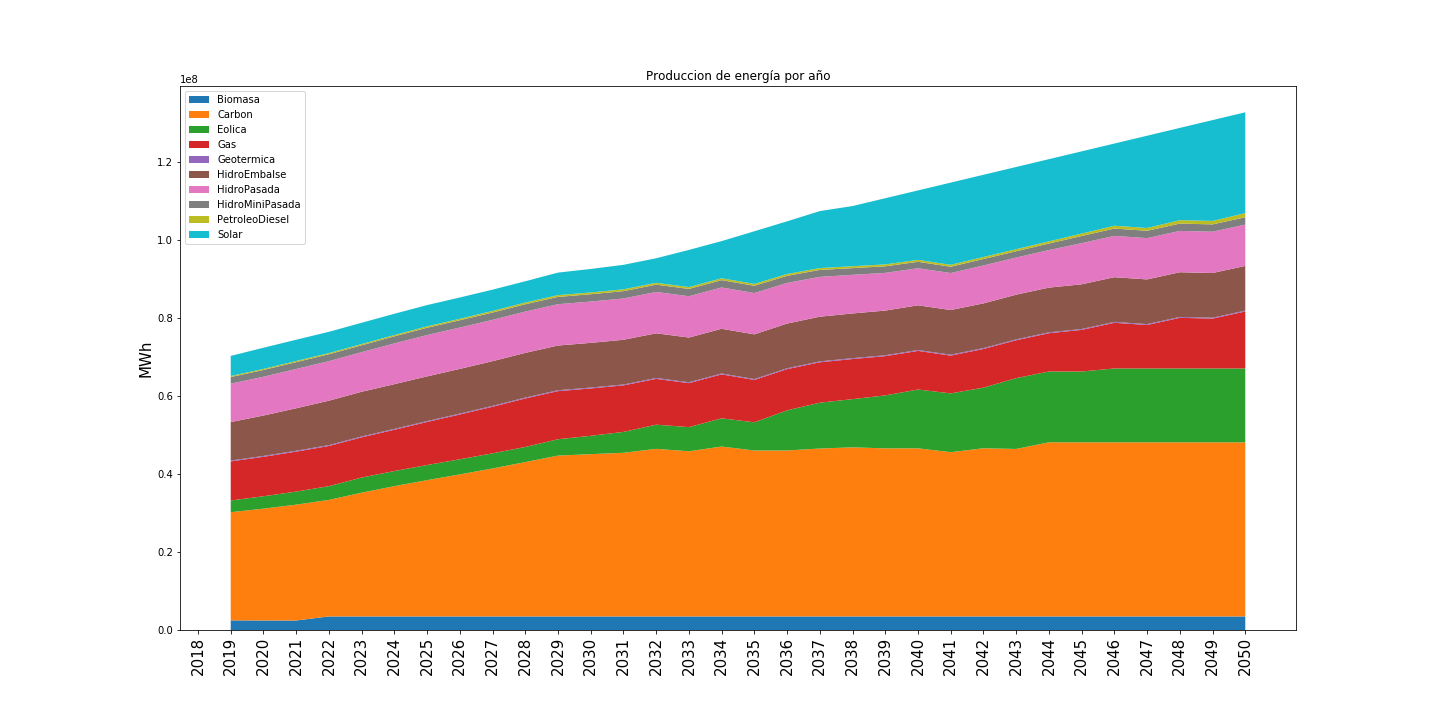
\includegraphics[width=\textwidth]{Apuntes/Figures/produccion_per_year_sin_cnt.png}
\caption{Energy production projected per technology by our model for the base year (2018) and the year range 2019-2050} \label{fig:modelbau}   
\end{center}
\end{figure}

\begin{figure}[ht!]
\begin{center}
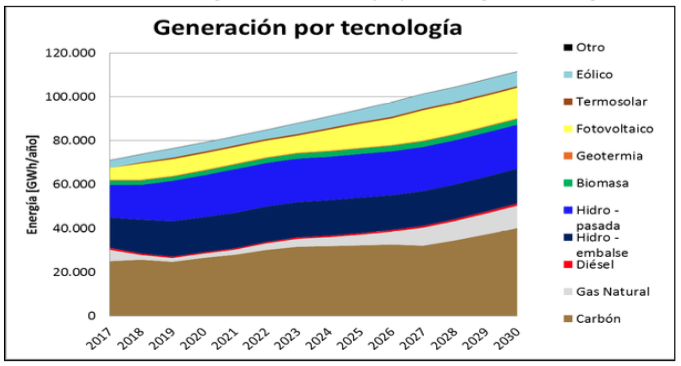
\includegraphics[width=13cm]{Apuntes/Figures/generadoras.png}
\caption{Projected energy production per technology made by Generadoras de Chile}
\label{fig:gener}
\end{center}
\end{figure}

\section{Chile's commitment in the Paris Agreement\footnote{https://climateactiontracker.org/countries/chile/2019-06-17/current-policy-projections/ \\https://mma.gob.cl/wp-content/uploads/2015/09/hojaderuta.pdf} }

\begin{itemize}
    \item By 2030: 30\% below 2007 GHG intensity of GDP (uncondicional target). This translates in 151\% above 1990 emissions excl. LULUCF by 2030. Figure \ref{fig:cap} shows the historical emissions and the projections until 2030 with data from the Climate Action Tracker analysis.
    \item By 2035: 60\% electricity production from renewable energy 
    \item By 2050: 70\% electricity production from renewable energy
    \item By 2024: close eight of the oldest coal-fired power plants (20\% of current coal electricity capacity) 
    \item By 2040: phase-out coal 
\end{itemize}



\subsection{Estimation of the CAP}
Based on Chile's pledge in the Paris Agreement, the projected total emissions up until the year 2030 are as shown in Figure \ref{fig:cap}, based on the data taken from the Climate Action Tracker (CAT) webpage. It should be noted that these emissions consider the main Greenhouse Gases (GHG)-- i.e $CO_2$, $CH_4$ and $N_2O$ -- transformed to their CO2 equivalent using IPCC conversion factors. In the Chilean case, the total emissions are dominated by $CO_2$ (78\%), followed by $CH_4$ with 12.5\% and $N_2O$  with 6\%. The remaining emissions are due to fluoride gases, which we will neglect in the following analysis. 

To determine the data, we take into account the fraction of emissions due to the electric sector, particularly energy generation. According to the Third Biennial Update Report about Climate Change\footnote{https://mma.gob.cl/wp-content/uploads/2018/12/3rd-BUR-Chile-SPanish.pdf}, the electric sector was responsible for the 35.1\% (36.25 $MtCO_2 e$) of the total emissions in 2016. We assume this fraction remains constant in the year interval 2019-2030. The total CAP estimated for the period is 462.24 $\rm  M t CO_2 e$.Figure \ref{fig:cap} shows the historical and projected emissions and the CAP determination. 


%\fel{Pia, este valir de 1113 es en toneladas equivalentes, por lo tanto tenemos 2 opciones. 1) Estimar el valor correspondiente a CO2 (no a otros GHG) y usar ese en nuestro modelo, o 2) Agregar todas los GHG que se consideran en este estimado a nuestro modelo (N2O, SO2, CO2, etc) para que el cap sea este numero. Espero tu cometario sobre esto.}




\begin{figure}[ht!]
 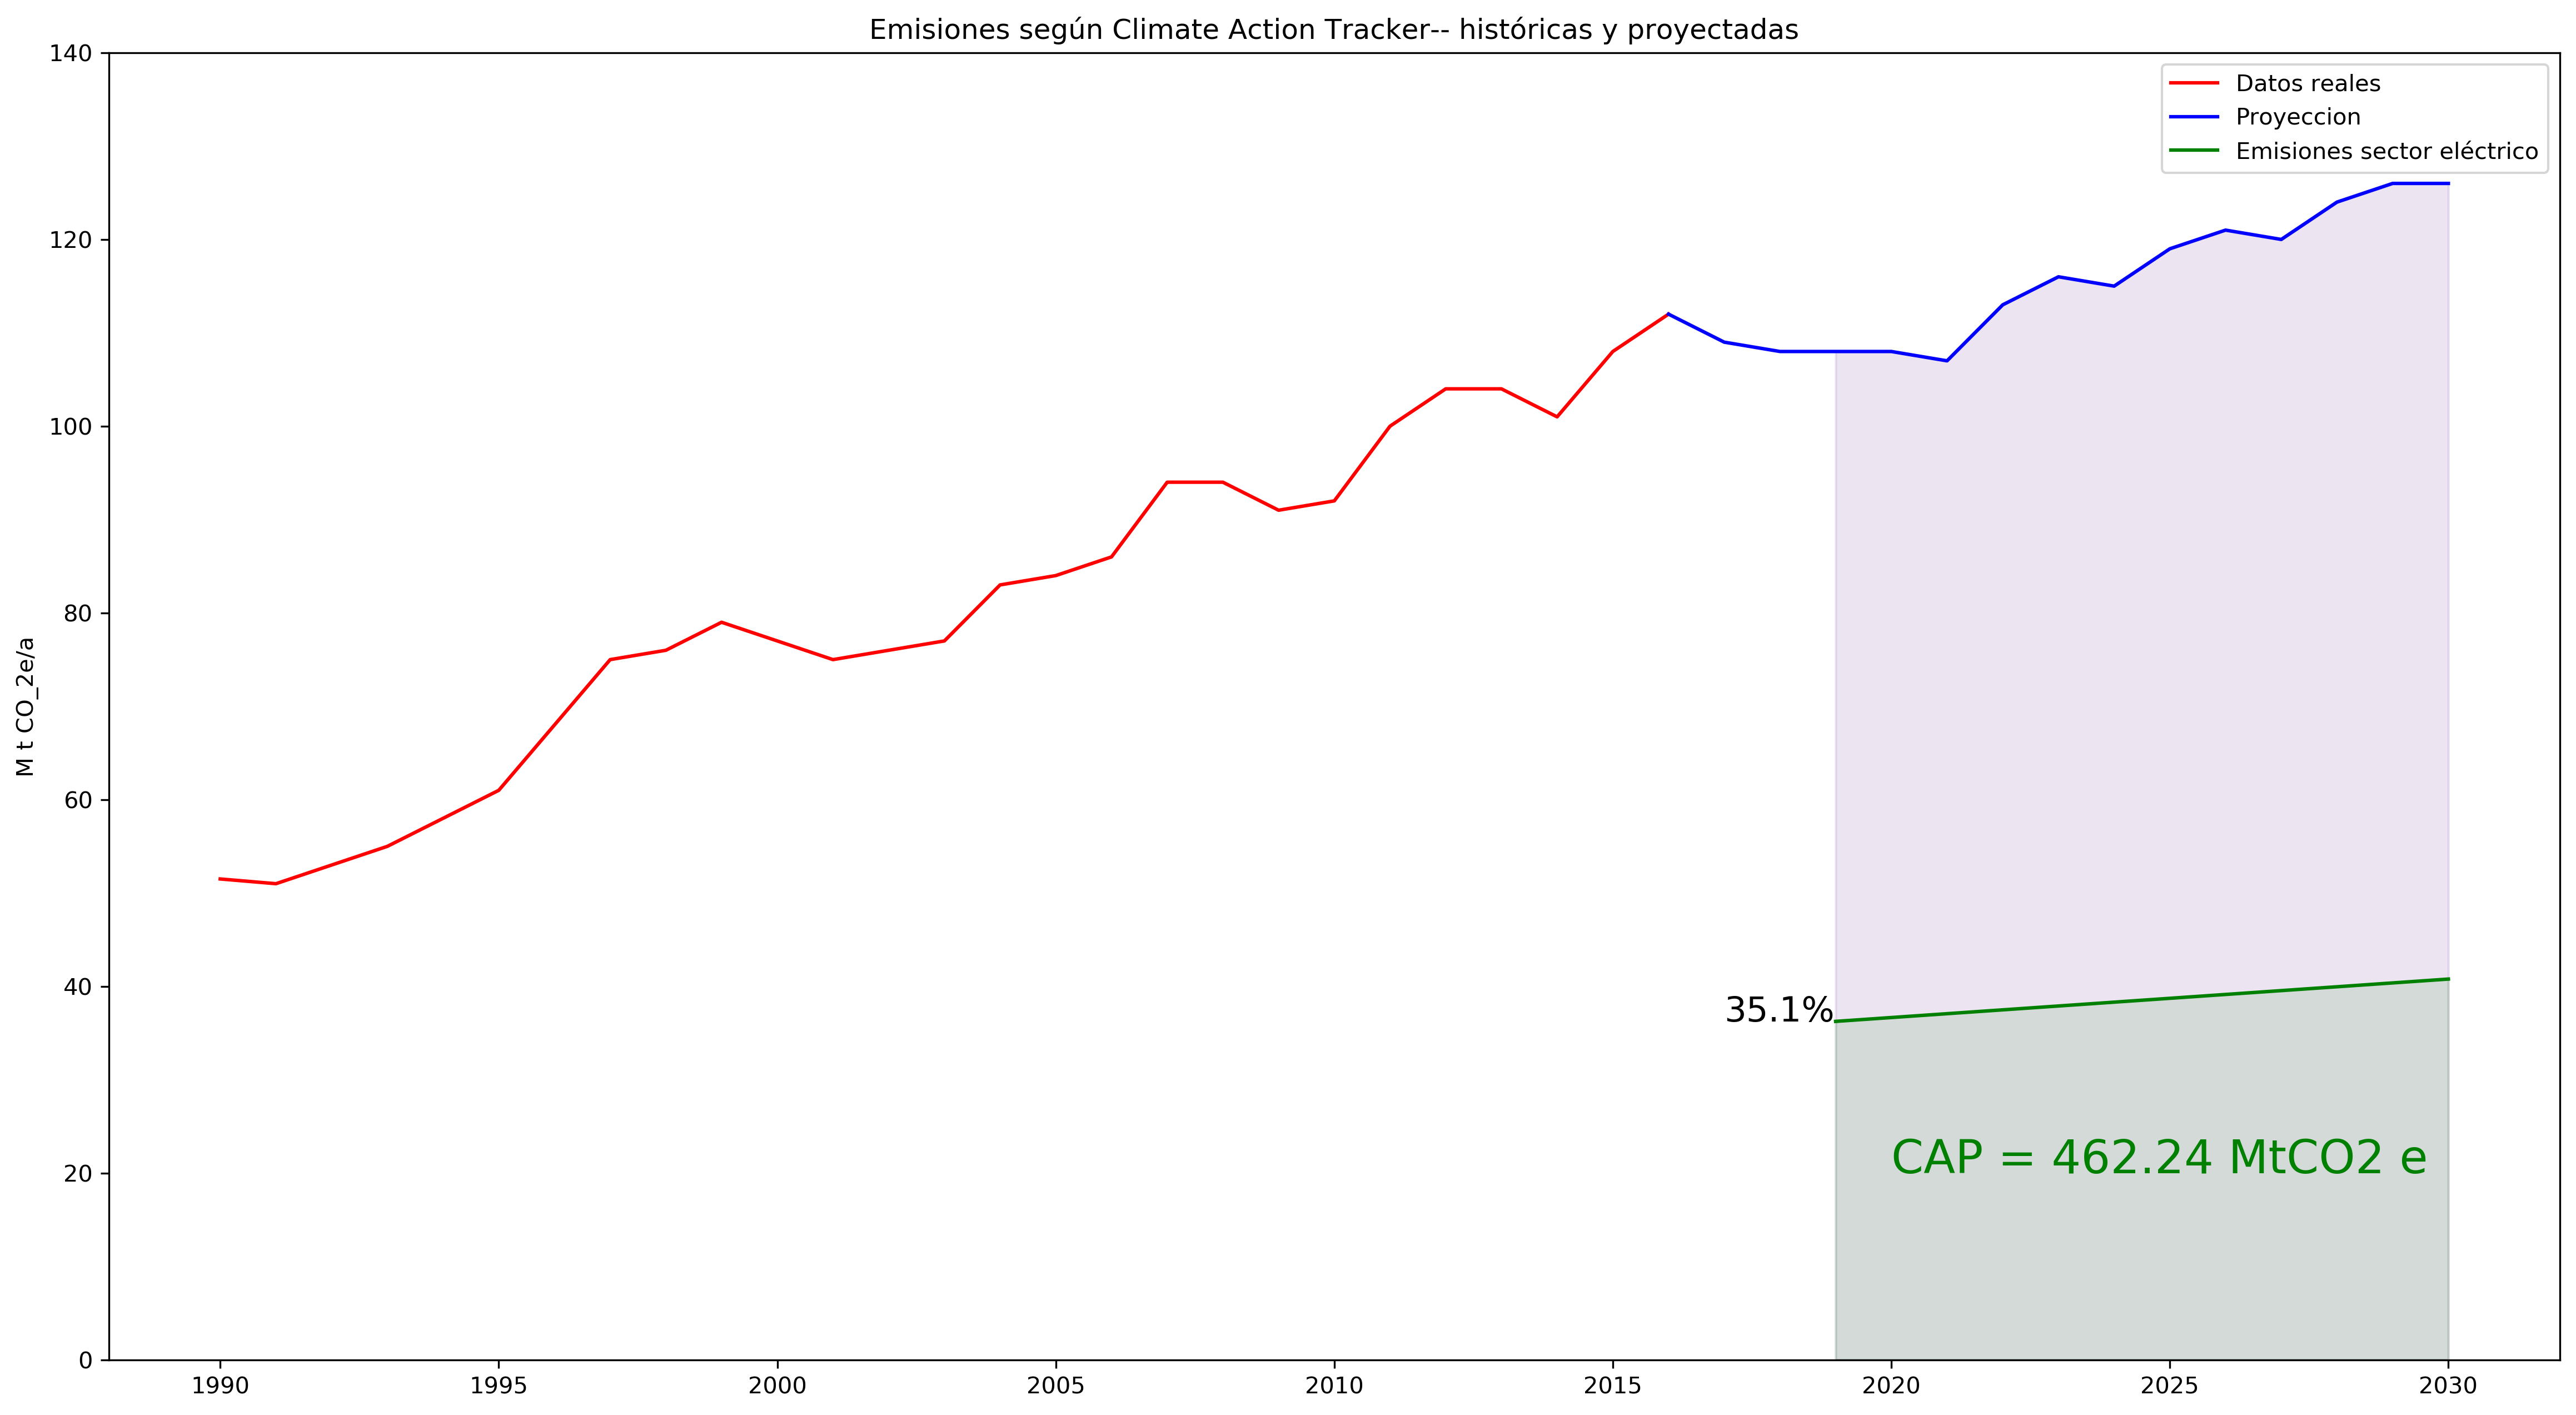
\includegraphics[width=\textwidth]{Apuntes/Figures/cap.png}
 \caption{Maximum emissions allowed in the 2019-2030 period for the chilean electric market. }
  \label{fig:cap}
  \end{figure}

\subsection{Cap and trade per year}

A variation of the cap and trade system is included in our model. Instead of a fixed cap for the entire period range, we now use an annual cap, and producers buy allowances on a yearly basis. The trading permit market also works per year. With these new considerations, the model is:

\underline{Producer's problem}

\begin{align}
\min_{(x_i,Q_i,A_i,P_i,V_i)} &  C_i(0, \pi^d(0),Q_i(0))+ I_i x_i(0) \nonumber \\ &+\sum_{\omega} Pr(\omega)   \Bigg( \sum_{t>0} \frac{1}{(1+R)^t} \Big[ (TC_i(t,\omega)\cdot C_i(t,\pi^d(t),Q_i(t,\omega) )  \nonumber \\
 & + \sum_{t > 0} TCR_i(t,\omega) \cdot I_i\cdot x_i(t,\omega) \Big] + \pia{A_i(t,\omega)\pi^a(t,\omega)+\pi^v(t,\omega)\cdot \Big(P_i(t,\omega)-V_i(t,\omega)\Big)} \Bigg)  \\
     \textrm{s.t \ } \nonumber
\end{align}
\begin{align}
    \Big(CF_i \cdot\tau\Big)  \Bigg[\bar{Q_i} + \sum_{t^{\prime}<\bar{t}} x_i(t^\prime,\omega) + x_i(0)+ \bar{Q}_i(t) \Bigg] - Q_i(t,\omega) & \geq 0  & \forall  \quad \omega, t  > 0 & \quad (\alpha_{i,t,\omega}) \\
    \Big(CF_i\cdot\tau \Big)\bar{Q_i}-Q_{i}(0) & \geq 0  &  \quad & \quad (\kappa_i) \\
\pia{A_i(t,\omega) - V_i(t,\omega) } & \geq  0  & \forall  \quad t,\omega & \quad (\beta_{i,t,\omega})\\
  \pia{ A_i(t,\omega) + \sum_{-i}P_{-i}(t,\omega) - V_i(t,\omega)-Q_i(t, \omega)\cdot \varepsilon_{i}} & \geq  0  &\forall \quad t,\omega & \quad (\gamma_{i,t,\omega})\\
 Q_i(0) & \geq  0 & \quad & \quad (\lambda_i)\\
 Q_i(t, \omega & \geq  0   & \forall  \quad \omega, t >0 & \quad (\delta_{i,\omega})\\
  x_i(0) & \geq  0 & \quad & \quad (\xi_i)\\
  x_i(t, \omega) & \geq  0   & \forall  \quad \omega, t >0 & \quad (\varphi_{i,\omega,t})\\
 RP_i - \bar{Q}_i - \bar{Q}_i(t) - x_i(0) - \sum_{t > 0} x_i(t,\omega)  &  \geq 0 &  \forall \quad i,\omega &  \quad (\psi_{i,\omega}) 
  \end{align}

\underline{Auctioneer's problem}
\pia{
\begin{align}
    \min_{\theta, \theta_2} & -\sum_{t,\omega} \theta(t,\omega) \pi^{a}(t,\omega) - \sum_{tau4,\omega} \theta_2 \pi_{ERNC}  & &  &\\
    \textrm{s.t \ } &  \phi^{-1}(M) \sigma^2 + \mu(t) - \theta(t,\omega) &  \geq & \quad 0  &\quad \quad  \forall  \quad t,\omega\\
    &  \theta(t,\omega)  & \geq & \quad 0 & \quad \quad  \forall \quad t,\omega\\
    & \theta_2(t,\omega) & \geq & \quad  \alpha D(tau4,\omega) & \quad \forall t \in tau4,\omega \\
    & \theta_2(t,\omega) & \geq & \quad 0 & \quad \forall t \in tau4,\omega 
\end{align}
}
\vspace{0.5cm}

\underline{Market clearing constraints:}

\begin{align}
\textrm{(available allowances)-- second stage}: &  \ \ \pia{ \sum_{i \in ernc} Q_i(t,\omega) = \theta_2(t,\omega)}    &   \forall \ t\in tau4, \ \ \omega & \ \ (\pi^{ernc}(t,\omega))\\
\textrm{(available allowances)-- second stage}: &  \ \ \pia{  \sum_{i} A_{i}(t,\omega) = \theta(t,\omega) }  &   \forall \ t,\omega & \ \ (\pi^{a}(t,\omega))\\
\textrm{(equilibrium in trading market)}: &   \ \  \sum_{i} P_i(t,\omega) = \sum_{i} V_i(t,\omega) & \forall \ t,\omega & \ \ (\pi^{v}) \\
\textrm{(fulfillment of the demand --first stage)}:  &   \ \  \sum_{i} Q_i(0) = D(0) &  & \ \ (\pi^d(0))\\
\textrm{(fulfillment of the demand --second stage)}:  &   \ \  \sum_{i} Q_i(t,\omega) = D(t,\omega), & \forall \ t,\omega & \ \ (\pi^{d,t}_\omega)
\end{align}


\begin{align}
    \mathcal{L}_i(x,Q,A,P,V) = &  C_i(0, \pi^d(0),Q_i(0))+  I_i x_i(0)  \nonumber \\ & +\sum_{\omega} Pr(\omega) \Bigg( \sum_{t>0} \frac{1}{(1+R)^t} \Big[ (TC_i(t,\omega)\cdot C_i(t,\pi^d(t),Q_i(t,\omega) )  \nonumber \\
 & + \sum_{t > 0} TCR_i(t,\omega) \cdot I_i\cdot x_i(t,\omega) \Big] + \pia{A_i(t,\omega)\pi^a(t,\omega)+\pi^v(t,\omega)\cdot \left(P_i(t,\omega)-V_i(t,\omega)\right) }\Bigg) \nonumber \\
 & +\sum_{\omega,t>0} \alpha_{i,\omega,t}\Bigg[  Q_i(t,\omega) - \Big(CF_i \cdot\tau\Big)  \Big(\bar{Q_i} + \sum_{t^{\prime}<\bar{t}} x_i(t^\prime,\omega) + x_i(0)+ \bar{Q}_i(t) \Big) \Bigg] \nonumber \\
 & +  \kappa_{i}\Big[Q_{i}(0)-\Big(CF_i\cdot\tau \Big)\bar{Q_i}\Big]  + \pia{\sum_{t>0,\omega}\beta_{i,t,\omega}\Big[  V_i(t,\omega)- A_i(t,\omega) \Big] }\nonumber \\
 & + \pia{\sum_{t>0,\omega}\gamma_{i,t,\omega} \Big[A_i(t,\omega) - \sum_{-i}P_{-i}(t,\omega) + V_i(t,\omega)+Q_i(t, \omega)\cdot \varepsilon_{i}\Big]} \nonumber\\
     & - \sum_{\omega, t>1}\delta_{i,\omega,t} Q_i(t,\omega) - \lambda_{i}\Big[Q_i(0)\Big] - \sum_{\omega, t>0}\varphi_{i,\omega,t} x_i(t,\omega) - \xi_i x_i(0) \nonumber \\
     & + \sum_{\omega}\psi_{i,\omega} \Big[  \bar{Q}_i+\bar{Q}_i(t) + x_i(0)  + \sum_{t > 0} x_i(t,\omega) - RP_i \Big]
\end{align}


The new KKT conditions to solve the equilibrium are:

\begin{align}
    I_i + \sum_{\omega}\psi_{i,\omega} -\sum_{\omega,\tau>1} \alpha_{i,\omega,\tau} -\xi_i & = 0 & \forall i {\color{blue}}&  \qquad (x_i(0))\\
    Pr(\omega) \Bigg[\frac{1}{(1+R)^t}TCR_i(t,\omega) \cdot I_i -  \varphi_{i,\omega,t}\Bigg] - \sum_{t> t\prime}\alpha_{i,\omega,t} ( CF_i \cdot \tau)  + \psi_{i,\omega}& = 0 & \forall i, \omega, t> 0  &  \qquad (x_i(t,\omega))\\
    (a_{i}+b_i Q_i(0))-\pi^d(0) + \kappa_i - \lambda_{i}  & = 0 & \forall i  &  \qquad (Q_i(0))\\
 Pr(\omega) \Bigg( \frac{1}{(1+R)^t}\Bigg) \bigg( (TC_i(t,\omega) \cdot a_{i}+b_i Q_i(t,\omega)-\pi^d(t,\omega) \bigg) + \alpha_{i,\omega,\tau} + \pia{\gamma_{i,t,\omega} \varepsilon_{i}} -\delta_{i,\omega,t} & =0 & \forall i, \omega, t>0 &  \qquad (Q_i(t,\omega)\\
  \pia{  Pr(\omega)\pi^a(t,\omega) - \sum_{t,\omega}\beta_{i,t,\omega} - \sum_{t,\omega}\gamma_{i,t,\omega} } & =0 & \forall i,t,\omega & \qquad (A_{i}(t,\omega)) \\
  \pia{  -Pr(\omega) \pi^v_{t,\omega} + \beta_{i,t,\omega}  + \gamma_{i,t,\omega}} & =0 & \forall i,t,\omega & \qquad (V_i(t,\omega)) \\
\pia{    Pr(\omega) \pi^v_{t,\omega} -\gamma_{t,\omega}} & = 0 & \forall i, t,\omega & \qquad (P_i(t,\omega))
\end{align}

\begin{flushleft}
Primal feasibility
\end{flushleft}

\begin{align}
    \Big(CF_i \cdot\tau\Big)  \Bigg[\bar{Q_i} + \sum_{t^{\prime}<\bar{t}} x_i(t^\prime,\omega) + x_i(0)+ \bar{Q}_i(t) \Bigg] - Q_i(t,\omega) & \geq 0  & \forall  \quad \omega, t  > 0 & \quad (\alpha_{i,t,\omega}) \\
    \Big(CF_i\cdot\tau \Big)\bar{Q_i}-Q_{i}(0) & \geq 0  &  \quad & \quad (\kappa_i) \\
\pia{A_i(t,\omega) - V_i(t,\omega) } & \geq  0  & \forall  \quad t,\omega & \quad (\beta_{i,t,\omega})\\
  \pia{ A_i(t,\omega) + \sum_{-i}P_{-i}(t,\omega) - V_i(t,\omega)-Q_i(t, \omega)\cdot \varepsilon_{i}} & \geq  0  &\forall \quad t,\omega & \quad (\gamma_{i,t,\omega})\\
 Q_i(0) & \geq  0 & \quad & \quad (\lambda_i)\\
 Q_i(t, \omega & \geq  0   & \forall  \quad \omega, t >0 & \quad (\delta_{i,\omega})\\
  x_i(0) & \geq  0 & \quad & \quad (\xi_i)\\
  x_i(t, \omega) & \geq  0   & \forall  \quad \omega, t >0 & \quad (\varphi_{i,\omega,t})\\
 RP_i - \bar{Q}_i - \bar{Q}_i(t) - x_i(0) - \sum_{t > 0} x_i(t,\omega)  &  \geq 0 &  \forall \quad i,\omega &  \quad (\psi_{i,\omega}) 
  \end{align}
  \begin{flushleft}
Complementary slackness
\end{flushleft}

\begin{align}
    \Bigg(\Big(CF_i \cdot\tau\Big)  \Bigg[\bar{Q_i} + \sum_{t^{\prime}<\bar{t}} x_i(t^\prime,\omega) + x_i(0)+ \bar{Q}_i(t) \Bigg] - Q_i(t,\omega)\Bigg) \cdot \alpha_{i,\omega,\tau} & = 0 & \forall  \quad \omega, t  > 0\\
    \Bigg(  \Big(CF_i\cdot\tau \Big)\bar{Q_i}-Q_{i}(0) \Bigg)\cdot \kappa_i & = 0  & \quad  \\
    \Bigg( \pia{ A_i(t,\omega) - V_i(t,\omega) } \Bigg) \cdot \beta_{i,t,\omega} & = 0 & \forall  \quad t>0 ,\omega\\
    \Bigg(  \pia{ A_i(t,\omega) + \sum_{-i}P_{-i}(t,\omega) - V_i(t,\omega)-Q_i(t, \omega)\cdot \varepsilon_{i}} \Bigg)\cdot \gamma_{i,t,\omega} & = 0 & \forall \quad t>0, \omega \\
    \Bigg( Q_i(0) \Bigg) \cdot \lambda_i & = 0 & \\
    \Bigg(Q_i(t,\omega)\Bigg ) \cdot \delta_{i,\omega} & = 0 & \forall  \quad \omega, t >0\\
    \Bigg( x_i(0) \Bigg) \cdot \xi_i & = 0 & \\
    \Bigg( x_i(t,\omega) \Bigg) \cdot \varphi_{i,\omega,t} & = 0 & \forall  \quad \omega, t >0 \\
    \Bigg(RP_i - \bar{Q}_i - x^{1}_i - \sum_{t>1} x^{t}_{i,w}  \Bigg) \cdot \psi_{i,\omega}&  = 0 &  \forall \quad i,\omega 
\end{align}

\begin{flushleft}
Dual Feasibility
\end{flushleft}

\begin{align}
    \alpha_{i,\omega,t} & \geq 0 \\
    \kappa_i & \geq 0 \\
    \beta_{i,t,\omega} & \geq 0 \\
    \gamma_{i,t,\omega} & \geq 0 \\
    \lambda_i & \geq 0 \\
    \delta_{i,\omega,t} & \geq 0 \\
    \xi_i & \geq 0 \\
    \varphi_{i,\omega,t} & \geq 0 \\
    \psi_{i,\omega} & \geq 0
\end{align}

For the Auctioneer, the Lagrangian function is 

\begin{equation}
    \mathcal{L}(\theta)=  -\Big(\sum_{t,\omega} \theta(t,\omega) \pi^{a}(t,\omega)\Big) -\pia{\Big( \sum_{t \in tau4, \omega}\theta_2(t,\omega)\pi^{ernc}(t,\omega)\Big)} + \sum_{t,\omega} \eta(t,\omega) \big(-\phi^{-1}(M) \sigma^2 - \mu(t) +\theta(t,\omega)\big) +
    \end{equation}
    \begin{equation}
    \pia{\sum_{t \in tau4, \omega} \eta_2(t,\omega)\Big(-\theta_2(t,\omega)+\alpha_t D(t,\omega)\Big)} -\zeta \theta(t,\omega) - \pia{\sum_{t \in tau4, \omega}\zeta_2(t,\omega)\theta_2(t,\omega)} \nonumber 
\end{equation}

The KKT equations for the auctioneer are:

\begin{align}
    -\pi^a(t,\omega)+\eta-\zeta & = 0 & \quad \big(\theta(t,\omega)\big)\\
    -\pi^{ernc}(t,\omega)+\eta_2(t,\omega)-\zeta_2(t,\omega) & = 0 & \quad \big(\theta_2(t,\omega)\big)\\
    \theta(0) & \geq  0 \\
    \theta(t,\omega) & \geq  0 \\
    \Big(\phi^{-1}(M) \sigma^2 + \mu(t) -\theta(t,\omega)\Big)\cdot \eta & =  0\\
    \eta & \geq  0\\
    \zeta & \geq 0
\end{align}



\begin{figure}[h!]
  \begin{subfigure}[b]{0.5\textwidth}
    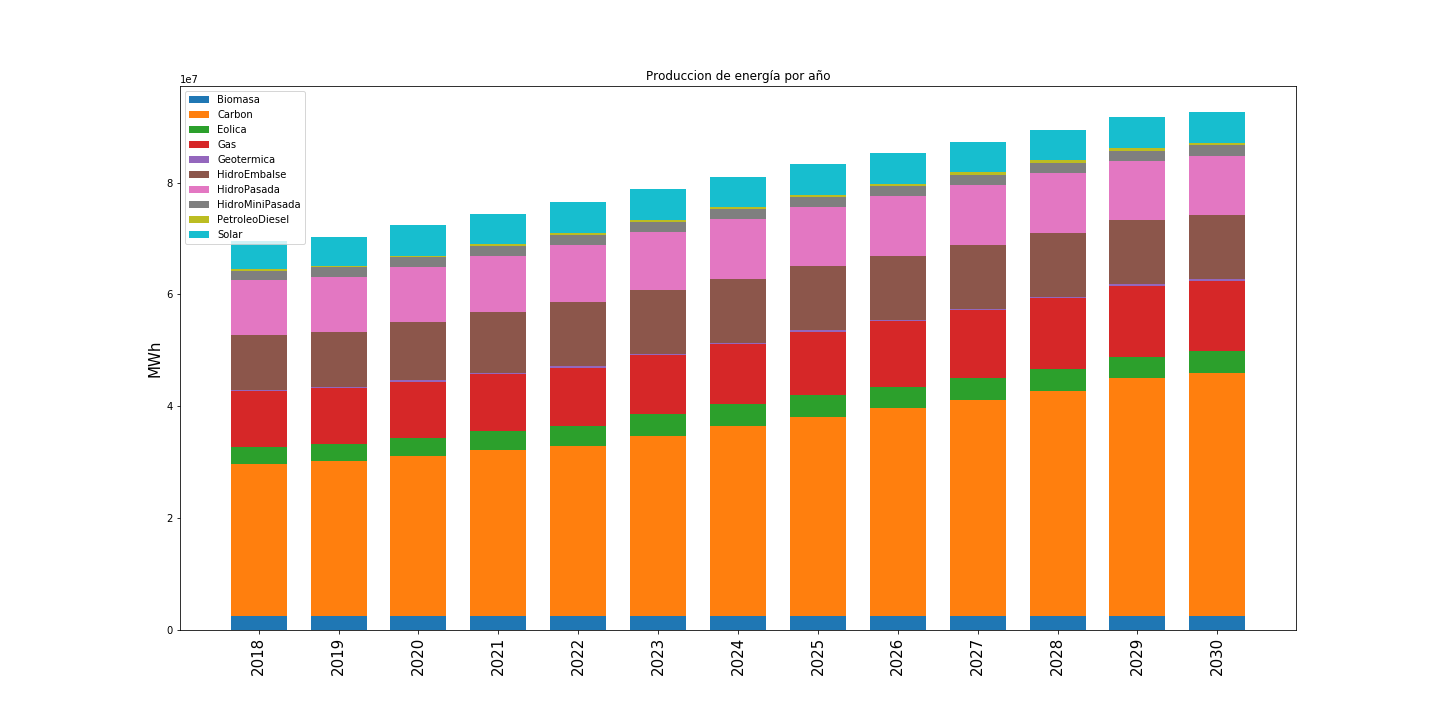
\includegraphics[width=\textwidth]{Apuntes/Figures/production_no_cnt_2030_annual.png}
    \caption{Production per year for each technology (producer) for the base-case (no cap and trade system)}
    \label{fig:2030nocnt_annual}
  \end{subfigure}\quad
  %
  \begin{subfigure}[b]{0.5\textwidth}
    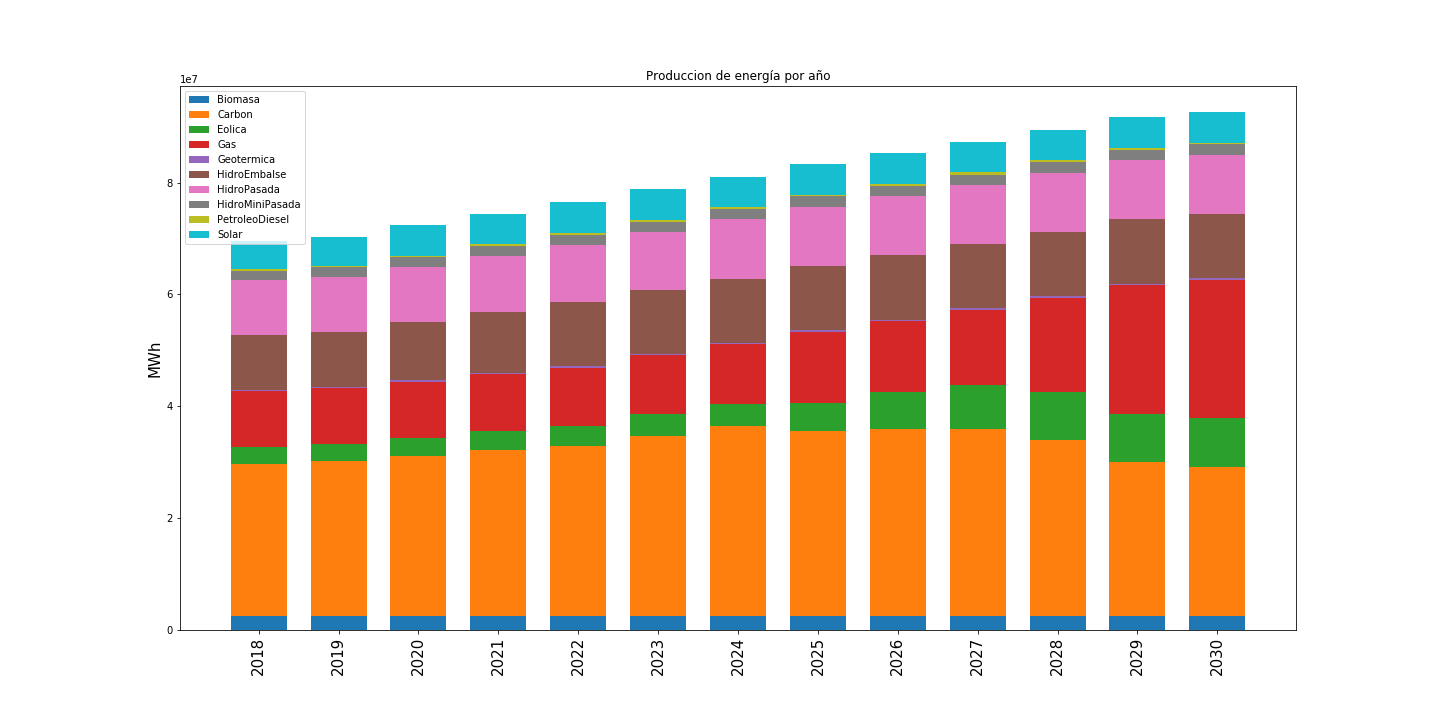
\includegraphics[width=\textwidth]{Apuntes/Figures/production_cnt_2030_annual.png}
    \caption{Production per year for each technology (producer) for the base-case (no cap and trade system)}
    \label{fig:2030cnt_annual}
  \end{subfigure}
\end{figure}


\section{Scenarios}
In each case, we compare each case with the current tax implemented, that is 5 $\rm USD/tCO_2$, a cap-and-trade scheme, and a mixture of both. 

\begin{itemize}
    \item Base-case: Bussiness as usual, no policies implemented. 
    \item CAP: Maximum number of allowances permited whithin a defined period
    
    \item Phase out coal by 2040
    
    \item 60\% of the energy generation based in NCRE by 2035

\end{itemize}




\begin{center}
 \begin{tabular}{ |c|c|c|c|c|  }
 \hline
 & CAP 2030 & Phase out coal by 2040 & 60\% from NCRE by 2035 & something 2050 \\ [0.5ex] 
 \hline\hline
Scenario 1 &  &    & &\\ 
 \hline
Scenario 2 & \xmark  &  &  &\\
 \hline
 Scenario 3 &  & \xmark & \xmark&\\
 \hline
 Scenario 4 &\xmark  &  &\xmark &\xmark\\
 \hline
Scenario 5 &\xmark  & \xmark & \xmark&\xmark\\ [1ex] 
 \hline
\end{tabular}
\end{center}



\end{document}

